
 
\hide{Beyond the physics of single hadrons described in the previous sections, the wealth of complexity embodied in the nuclear landscape emerges from QCD and the other forces of the SM. The first steps in addressing this complexity from LQCD have been made over the last decade, and we anticipate that LQCD will be an increasingly important part of nuclear theory in the coming years. Since the SM forms the foundation of nuclear physics, LQCD can be used to study the forces that bind nucleons into nuclei and govern their interaction, as well as to investigate how nuclear systems interact with external electroweak and possible physics beyond the Standard Model.}

\subsection{Nuclear spectroscopy}

Determining the ground state energies and binding energies of light nuclei is a central challenge. The very first QCD calculations of nuclei less than a decade old and significant advances in the study of nuclear systems have occurred over the last five years.
The first calculations of bound systems with baryon number $A\ge2$ were of the doubly-strange $H$-dibaryon system at unphysical quark masses
\cite{Beane:2010hg,Inoue:2010es,Beane:2011xf}. Additional calculations have ensued \cite{Beane:2012vq,Yamazaki:2012hi,Yamazaki:2015asa}, with almost physical quark mass calculations being currently performed by the PACS-CS collaboration \cite{}. Of particular note

Nuclear systems are particularly challenging for LQCD for multiple reasons. As emphasised by Parisi and Lepage \cite{Lepage:1989hd,Parisi:1983ae,Hamber:1983vu}, single baryon correlation functions exhibit a signal-to-noise ratio that degrades exponentially with the temporal separation. FOr nuclear systems, the problem only becomes more challenging \cite{Beane:2009kya,Beane:2009gs}. Extraction of the eigen-energies is consequently challenging. A number of methods have been developed that aim to ameliorate this issue, either defining better-behaved estimators \cite{Beane:2014oea,Wagman:2017gqi,Wagman:2017xfh,Wagman:2016bam} or new analysis strategies that optimize the ratio of signal to noise \cite{Detmold:2014hla}. None of these methods has completely solved the noise problem, but have proved sufficient for studies of the lightest few nuclei. 

The first calculations of bound nuclear states in QCD have been performed by the NPLQCD collaboration \cite{} and the PACS-CS collaboration (bound states have also been found using HAL potential method \cite{} based on Refs.~\cite{}, although it is only recently that systematics have begun to be addressed in this method \cite{}). Bound states have been studied over a range of quark masses and atomic numbers with a recent review of these results is presented in Ref.~\cite{}. These calculations have been used as input in effective field theory analyses that extend the reach of LQCD calculations to larger nuclei \cite{Barnea:2013uqa,MORE}.

\subsubsection{Future directions}
There are many opportunities for increased effort in this area as well as many technical challenges that exist in going to larger systems and performing calculations at the physical quark masses. 
Extending existing calculations to even moderately larger $A$ will have significant impact as nuclei that require $p$-shell configurations become accessible. These systems depend on more complicated aspects of hte nuclear forces than the $A\le4$ nuclei that have been studied and new lattice calculations will be useful in constraining different spin and isospin components of these forces. Larger nuclei also exhibit interesting collective effects such as halo structures (eg,  ${}^{6,8}$He), cluster structures (eg ${}^{8}$Be, ${}^{12}$C) and deformations that would be very instructive to see emerge from LQCD calculations. Additionally, LQCD offers the possibility of investigating nuclei away from the physical quark masses, or for different gauge and fermion content of the theory, as an intellectual pursuit of its own in which questions related to the naturalness of nuclear physics \cite{Orginos:2015aya}. Calculations in this direction using $N_f=N_c=2$ appear in Refs.~\cite{Detmold:2014qqa,Detmold:2014kba}.

For bound nuclear systems there are two exponentially difficult algorithmic challenges that must be addressed. The complexity of contractions grows 
facorially with the system size, at least naively; calculations for $^4$He are naively $6!6!/2\sim 260,000$ more difficult than for a proton. Efforts to reduce these costs have enabled the progress described above and have proceeded via construction of enumerative \cite{Doi:2012xd,Gunther:2013xj} and recursive \cite{Detmold:2012eu} algorithms. 


\subsection{Nuclear Structure}
\label{sec:nuclearstructure}

Nuclei are complex objects and exploration of their structure from the underlying quark and gluon degrees of freedom offers challenges and opportunities for new calculations. On the one hand, the spectroscopy and decay channels of excitations of nuclei are an important source of structure information. On the other hand, interactions of nuclei with electroweak probes also contribute much to the phenomenological information we have about nuclear structure. 
In particular, the magnetic moments,  higher multiple moments and polarizabilities  enable a static picture of nuclei to be determined. The corresponding form factors reveal charge and current distributions in nuclei and  have lead to the 
development of our understanding of nuclear structure. 
Nuclear parton distributions provide further information on the substructure of nuclei as seen from boosted processes such as deep-inelastic scattering, and have historically been one of the 
most striking examples of an arena in which non-nucleonic degrees of freedom are important inside the nucleus. The EMC effect \cite{Aubert:1983XX}, discovered in 1983, shows that the distribution of quarks and gluons in a nucleus is different from the incoherent sum of the distribution in the nucleon.

From the LQCD point of view, only the first steps have been taken in this direction, with isovector magnetic moments \cite{Beane:2014ora,Beane:2015yha,Detmold:2015daa} and magnetic  polarizabilities \cite{Chang:2015qxa} of nuclei up to $A=4$ being computed at heavier than physical quark masses using background field methods. Interestingly, relations that exist between magnetic moments in phenomenology are also apparent in the LQCD resutls at heavy quark masses. For example,  the magnetic moment of the triton is very close to the magnetic moment of the neutron as in the simplest shell-model configuration, the two protons spin pair to zero. The extracted magnetic moments and polarizabilities are summarized in Fig.~\ref{fig:summaryBETA} and as seen in left panel, the close agreement between the LQCD  and experimental magnetic moments is striking.
%
\begin{figure}[!t]
	\centering
	\raisebox{0.1\height}{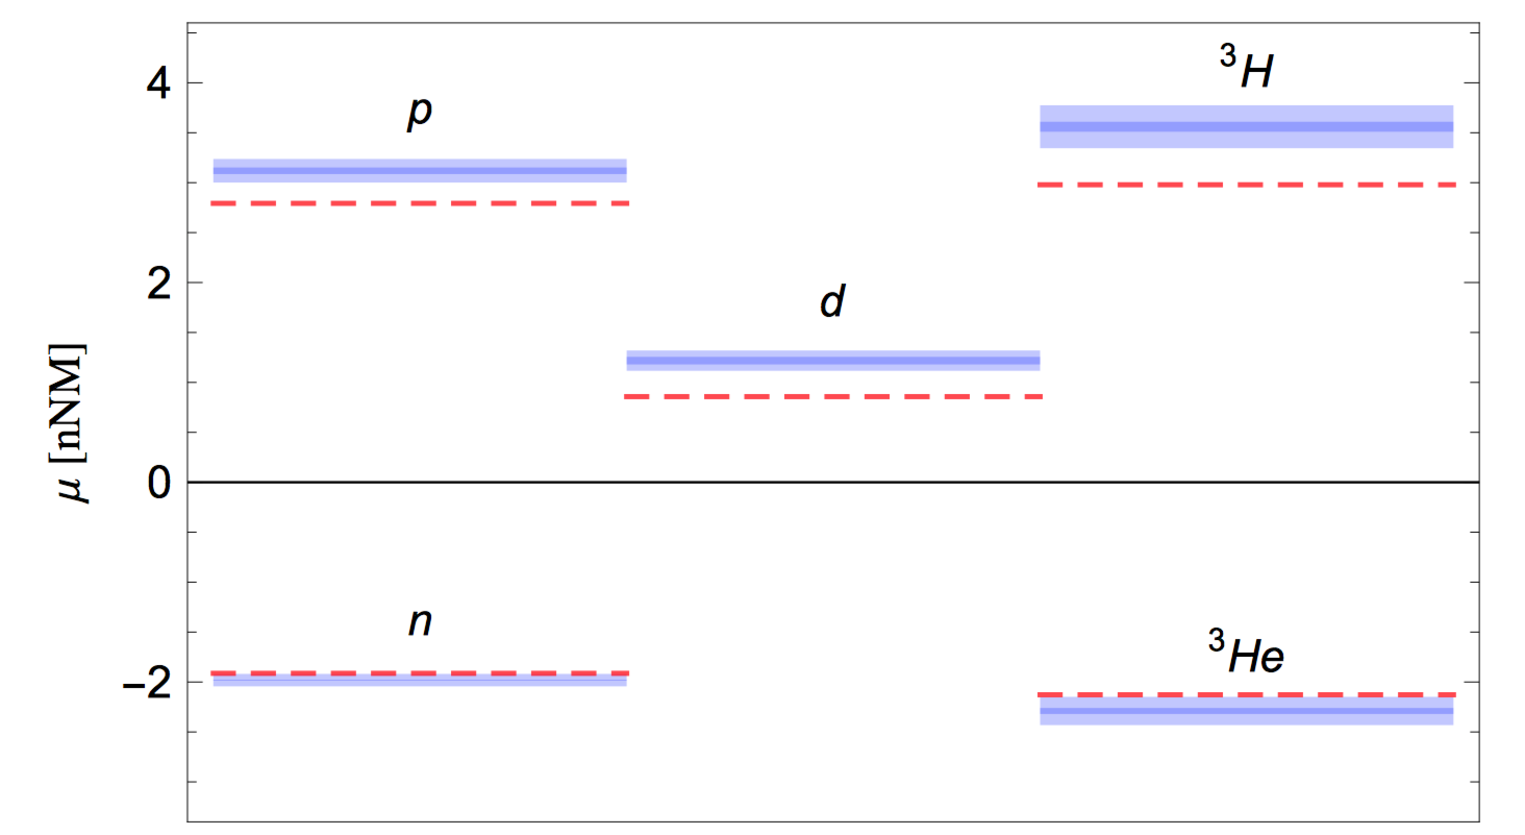
\includegraphics[width=0.48\columnwidth]{figures/MagMoms.pdf}  }
	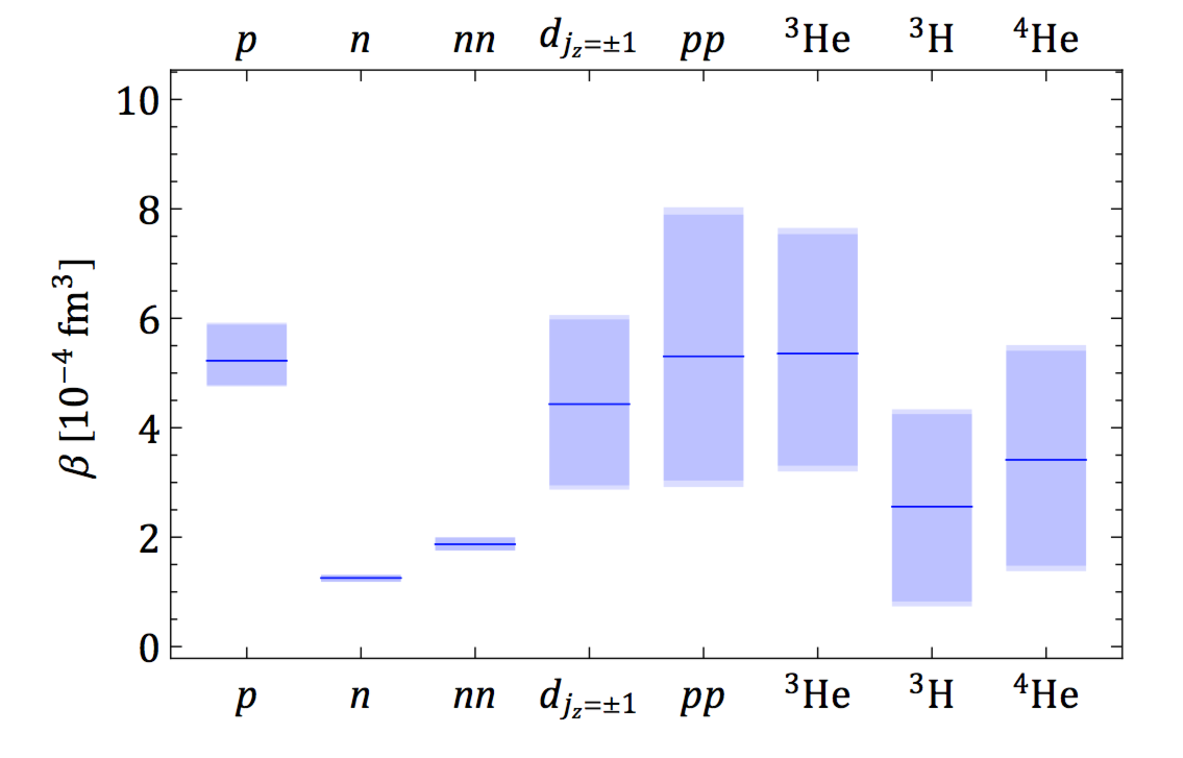
\includegraphics[width=0.49\columnwidth]{figures/PhysPols.pdf}
	\caption{ 
		A summary of the magnetic moments~\protect\cite{Beane:2014ora} (left panel) and polarizabilities (right panel) of the nucleons and
		light nuclei calculated with LQCD at a pion mass of
		$m_\pi\sim 805~{\rm MeV}$~\protect\cite{Chang:2015qxa}.    }
	\label{fig:summaryBETA}
\end{figure}

%
\begin{wrapfigure}{r}{0.5\columnwidth}
	\vspace*{-0cm}
	\centering
	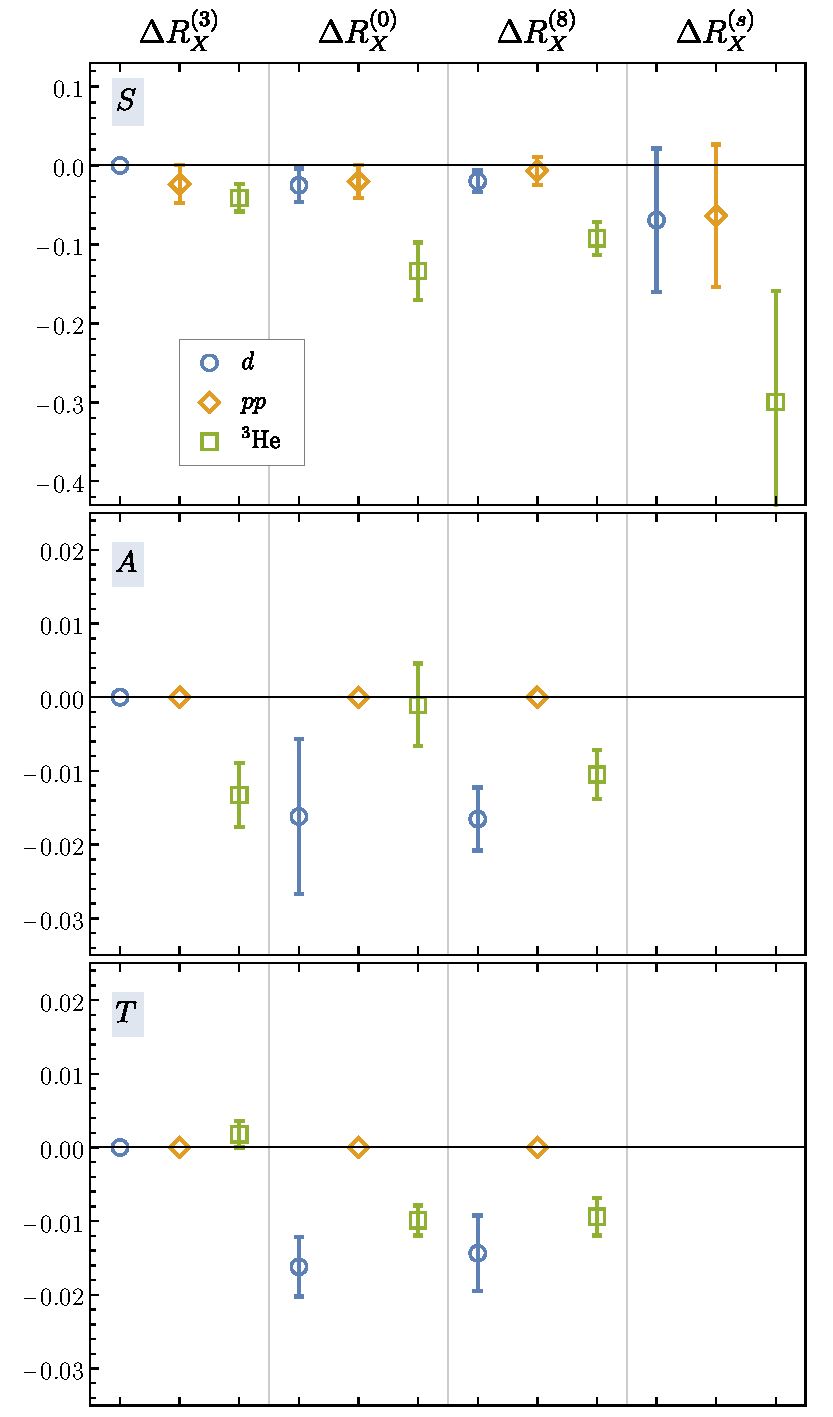
\includegraphics[width=0.4\columnwidth]{figures/RatioSummary.pdf}  
	\caption{ 
		The differences of the scalar, axial and tensor current matrix elements of light nuclei from single particle expectations ~\protect\cite{Beane:2015yha}. Nuclear effects can be identified by the deviation of quantities from zero.   
	}
	\label{fig:SAT}
	\vspace*{-1.5cm}
\end{wrapfigure}
%
The Gamov-Teller (GT) contribution to the weak decay of the triton \cite{Savage:2016kon} and the coupling on $A\le3$ nuclei to scalar and tensor currents \cite{Chang:2017eiq} has also been investigated using similar background field techniques. The weak decay of the triton is the simplest nuclear probe of weak interactions and the GT contribution is most uncertain. 
As discussed extensively in the companion White Paper on Fundamental Symmetries, the scalar current is relevant for interactions with nuclei in many models of dark matter~\cite{Undagoitia:2015gya} and for searches for new physics in precision spectroscopy~\cite{Delaunay:2016brc,Delaunay:2017dku}, while the tensor current determines 
the quark electric dipole moment contribution to a nuclear electric dipole moment~\cite{Engel:2013lsa,Yamanaka:2016umw,Chupp:2017rkp} and is thus an important ingredient in searches for new sources of time-reversal violation. 
 The nuclear dependencies of the various currents are shown in Fig.~\ref{fig:SAT}.


While the quark structure of nucleons and nuclei is relatively well probed by electron scattering experiments, unraveling the gluonic structure is vastly more difficult. The Electron Ion Collider \cite{Accardi:2012qut}, a major new Nuclear Physics accelerator facility planned for construction in the 2020s, will particularly target the gluon structure of nucleons and nuclei. LQCD calculations can play an important role in planning this facility and setting benchmarks for first measurements of various gluon structure quantities. To this end, a preliminary study of the modification of the lowest moment of the unpolarized  gluon distributions in nuclei, the gluon momentum fraction, has been performed \cite{Winter:2017bfs}  although nuclear effects were bounded rather than resolved.   In addition, the first moment of the gluon transversity structure function was investigated in the spin-1 deuteron. This latter  quantity  corresponds to a target helicity flip by two units and so vanishes for the nucleon; it is therefore intrinsically a nuclear effect.




\subsubsection{Future directions}

%SPECTROSCOPY
Applying the variational techniques discussed in Section \ref{sec:hadronspectroscopy} to nuclear systems will allow at least some of the low energy excitations of nuclei to be resolved given sufficient computational resources. By using a large basis of operators of different symmetries and structures, this will allow a detailed understanding the nature of these excitations and the origin of collectivity in nuclei. Such calculations will also provide insight into how nuclear structure changes with the parameters of the Standard Model.

%FORM FACTORS
Calculations of electroweak interactions with nuclei that include recoil from the currents and thereby determine the input nuclear form factors necessary to constrain  elastic  neutrino-nucleus scattering. This will reduce the theoretical uncertainties inherent in the coming long-baseline neutrino experimental program. Coupled to the calculations of the proton charge radius described above, calculations of the charge radii of the light nuclei $d$, $^3$He and $^4$He  will enable further insight into the discrepancies in nuclear charge radii between muon spectroscopy and electro scattering and spectroscopy \cite{}.


%PARTON
Future calculations will explore the modification of moments of parton distributions in light nuclei, thereby probing the EMC effect from QCD. While these calculations will be in light nuclei, effective field theory \cite{Chen:2004zx,Chen:2016bde} and phenomenology \cite{Hen:2016kwk} suggest that two-body correlations that can be determined in the few nucleon sector are sufficient to describe the EMC effect. LQCD can also help address more complex questions such as the flavor and spin dependence of the EMC effect that are hard to access from phenomenology. Using the techniques described in Section \ref{sec:hadronstructure}, the Bjorken-$x$ dependence of nuclear parton distributions will also be accessible, significantly expanding the connection of LQCD to phenomenology in this area. Further calculations of gluon ic properties will reveal exotic aspects of nculear structure such as double-helicity-flip parton distribtions.



%\begin{itemize}
%	\item Explore nuclear modification of hadron structure. Modifications of charges, form factors, moments of PDFs  (derive the EMC effect from QCD). 
%	Do this with complete flavour breakdown
%	\item Determine spatial pictures of nuclei from ``charge distributions''' as Fourier transforms of various form factors. Radii
%	\item Study $x$-dependent PDFs, gluonic aspects of hnuclear structure
%	\item Exotic glue
%\end{itemize}



\subsection{Nuclear interactions}

\begin{itemize}
	\item Scattering  phase shifts of $NN$ systems. validation of LQCD calculations at physical point. Understanding role of Coulomb, eg $a_{pp}$ vs $a_{np}$ vs $a_{nn}$ in the spin singlet channel.
	\item Scattering phase shifts for  hyperon-nucleon and hyperon-hyperon systems. Input to nuclear equation of state (EoS) for potential hyperonic matter in neutron stars; connection to NS-NS mergers and NICER.
	\item Three and four body forces. Experimental constrain in particular on $nnn$ interactions is poor but increasingly relevant in larger nuclei. Most direct constrain is from EFT matching to finite volume energy levels computed in LQCD. Multiple EFT groups using unphysical mass lattice calculations to do this right now:LANL, Hagen/ORNL (pion-full), Lovato/Pederiva, Van Kolck using different EFT formulations

\end{itemize}


SCATTERING PHASE SHIFTS





\begin{wrapfigure}{r}{0.5\columnwidth}
	\centering
	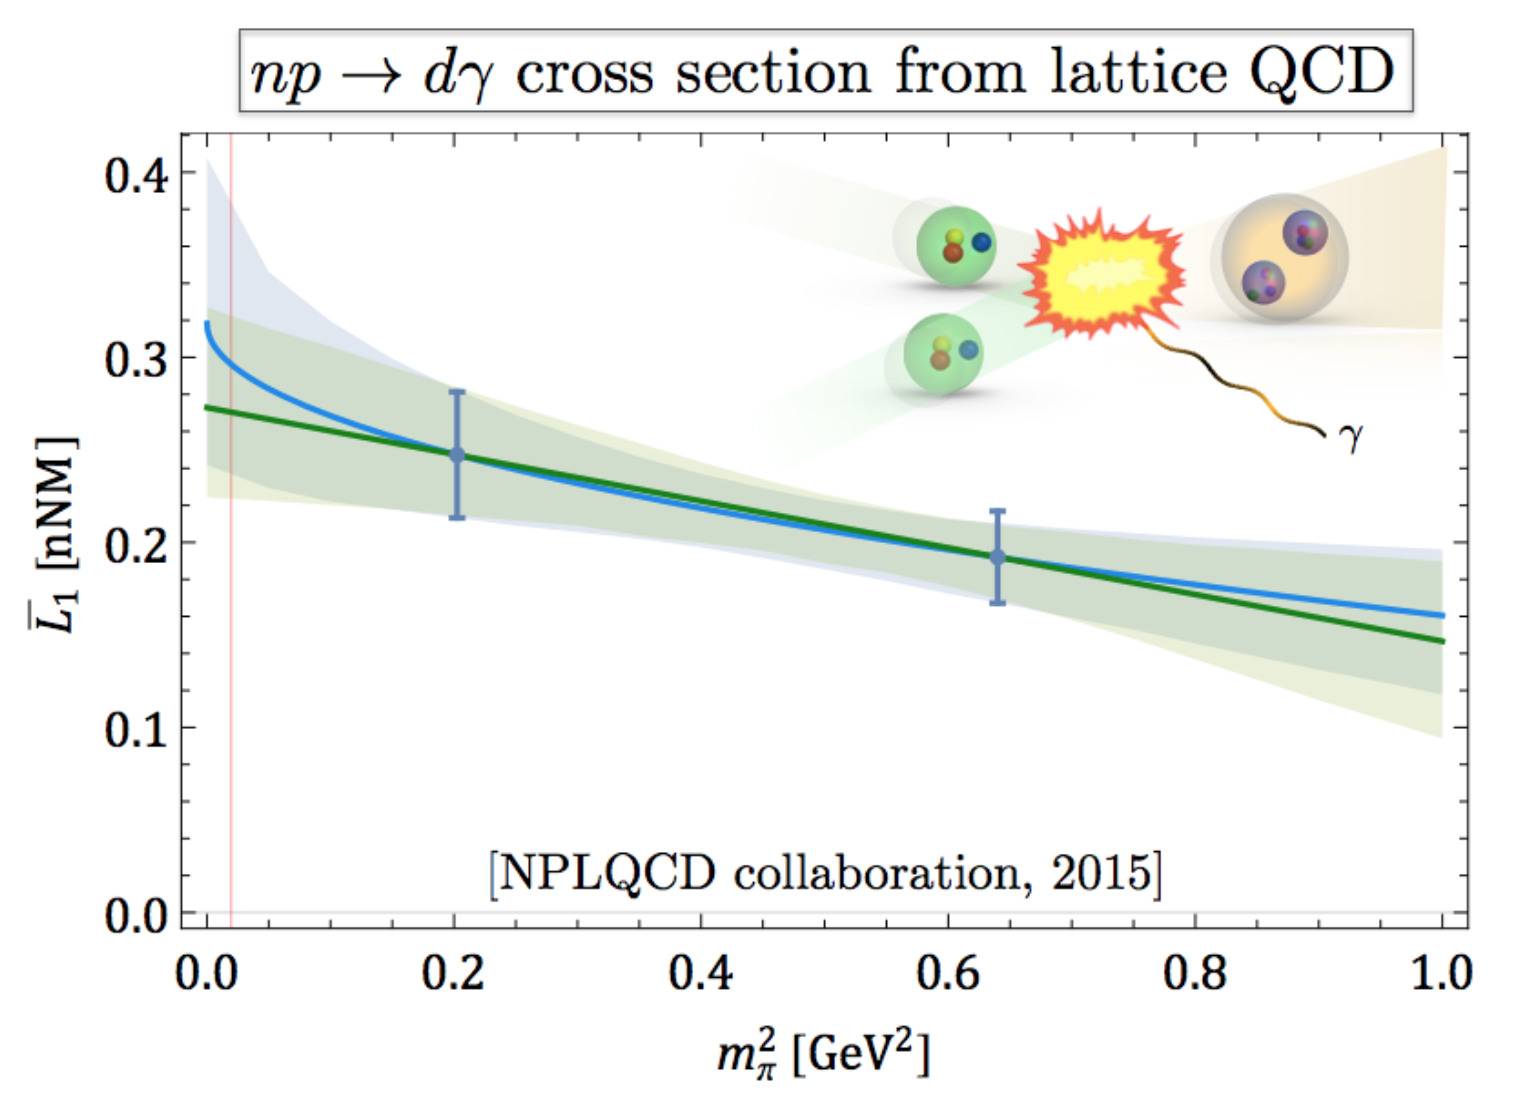
\includegraphics[width=0.48\columnwidth]{figures/npTOdgamma.png}  
	\caption{ 
		The short-distance correlated two-nucleon (meson-exchange current)
		contribution to $np\rightarrow d\gamma$~\protect\cite{Beane:2015yha}.    
	}
	\label{fig:L1bar}
	\vspace*{-0.4cm}
\end{wrapfigure}
%
Calculations of two-nucleon systems in external magnetic fields were used to isolate the
short-distance two-body electromagnetic contributions to the low-energy radiative capture process $np\rightarrow d\gamma$,
and the photo-disintegration processes $\gamma^{(*)}d\rightarrow np$~\cite{Beane:2015yha},
as shown in Fig.~\ref{fig:L1bar}. 
In nuclear potential models, such contributions are described by 
phenomenological meson-exchange currents; using LQCD we were able to determine them directly from the quark and gluon interactions of QCD.
This was achieved by calculations of coupled neutron-proton systems in multiple background magnetic fields, at two values of the 
quark masses, corresponding to pion masses of $m_\pi\sim 450$ and 806 MeV. The results were extrapolated to the physical pion mass using pionless EFT, allowing the rate of the low-energy inelastic process to be determined 
at the physical point. 
%Extrapolating to the physical pion mass,
%a cross section of $\sigma^{\rm lqcd} (np\rightarrow d\gamma)=\sigmaPHYS~{\rm mb}$ 
%was obtained 
%at an incident neutron speed of $v=2,200~{\rm m/s}$, consistent with the experimental value of
%$\sigma^{\rm expt}(np\rightarrow d\gamma)=\sigmaEXPT~{\rm mb}$.
%
%
This is the first LQCD calculation of an inelastic nuclear reaction and both it, along with an extension to investigate strong magnetic fields, appear 
in {\it Physical Review Letters}~\cite{Beane:2015yha,Detmold:2015daa}. 




ed the first LQCD calculations of the nuclear matrix element determining the $pp\rightarrow d e^+\nu_e$ fusion cross section and the Gamow-Teller matrix element contributing to tritium $\beta$ decay. The method used is very similar to the one that will be needed to achieve the objectives of this proposal.
Using a new implementation of the background field method,
the matrix elements were calculated at the SU(3)-flavor symmetric 
value of the quark masses, corresponding to a pion mass of $m_\pi\sim 806~{\rm MeV}$. 
The Gamow-Teller matrix element in tritium is found to be $0.979(03)(10)$ at these unphysical quark masses, 
which is within $2\sigma$ of the experimental value. 
Assuming that the short-distance correlated two-nucleon contributions to the matrix element 
(meson-exchange currents) depend only mildly on the quark masses, as seen for the analogous magnetic interactions, 
the calculated $pp\rightarrow d e^+\nu_e$ transition matrix element leads to a fusion cross section at the physical quark 
masses that is consistent with its currently accepted value, although further calculations are required to  better substantiate this conclusion. Moreover, the leading two-nucleon axial counterterm of pionless EFT is determined to 
be $L_{1,A} = 3.9(0.2)(1.0)(0.4)(0.9)~{\rm fm}^3$ at a renormalization scale set by the physical pion mass, 
also in agreement with the accepted phenomenological range. 
This work concretely demonstrates that weak transition amplitudes in few-nucleon systems can be studied directly 
from the fundamental quark and gluon degrees of freedom and  
opens the way for future investigations of many important quantities in nuclear physics. 
This work appeared in {\it Physical Review Letters} \cite{Savage:2016kon} in 2017 and was the subject of a DOE Office of Science highlight and an APS synopsis.\footnote{See {\tt https://science.energy.gov/np/highlights/2017/np-2017-12-b/} and \\{\tt https://physics.aps.org/synopsis-for/10.1103/PhysRevLett.119.062002}.}







For some specific nuclei such as germanium, single $\beta$ decay is energetically forbidden, but double $\beta$ decay is allowed. In the Standard Model, this decay occurs with the release of two electrons and two anti-neutrinos, conserving lepton number  ($2\nu\beta\beta$-decay). In many beyond the standard model scenarios, either with light Majorana neutrinos (particles that are their own antiparticles) or with other forms of lepton number non-conservation at high scales,  a second form of  double $\beta$ decay that involves no neutrinos in the final state ($0\nu\beta\beta$-decay) can occur. Observation of this latter process would be an unambiguous signal for new physics. Understanding of the implications of such an observation, as well as design of future experiments seeking this decay mode, requires understanding the relevant $\Delta I=2$ nuclear transition matrix elements. This is a challenging task and state-of-the-art nuclear theory calculations differ by an order of magnitude. LQCD offers the prospect of providing useful input in this area through calculations of the relevant matrix elements in light nuclei that can be used to control uncertainties in nuclear models. In the last two years, the $2\nu\beta\beta$ process has been studied in the $pp\to nn$ transition \cite{Tiburzi:2017iux,Shanahan:2017bgi},  the pionic matrix elements, $\langle \pi^+ | {\cal O} | \pi^- \rangle$, of $\Delta I =2$ short distance operators \cite{Nicholson:2018mwc}, and the $\pi^-\to \pi^+ e^- e^-$ and $\pi^-\pi^-\to e^-e^-$ transitions induced  by a light Majorane neutrino \cite{Feng:2018pdq,Murphy2018ICHEP}, have all been investigated for the first time. Future refinements of these calculations, even restricted to few nucleon systems, have the potential to significantly impact experimental search design.  Already  these finding suggests that nuclear models for neutrinoful and neutrinoless $\beta\beta$ decays need to incorporate this previously neglected contribution if they are to provide reliable guidance for next-generation neutrinoless $\beta\beta$-decay searches. 




\subsection{Nuclear input for neutrino physics and fundamental symmetries}


Nuclei are used as targets in intensity frontier experiments that are trying to probe the neutrino sector and to look for physics beyond the SM. In particular, argon ($Z=18$) is the target material for a number of current neutrino experiments and will be the target for the upcoming Deep Underground Neutrino Experiment (DUNE), while a range of nuclei such as sodium ($Z=11$), xenon ($Z=54$) are used in dark matter direct detection experiments \cite{Undagoitia:2015gya}. Charge lepton flavor violation searches look for $\mu\to e$ conversion in the field of aluminium ($Z=13$) \cite{Albrecht:2013wet}, and precision isotope-shift spectroscopy experiments consider a wide range of nuclei ranging from hydrogen ($Z=1$) to ytterbium ($Z=70$) in  order to constrain new physics \cite{Delaunay:2016brc,Delaunay:2017dku}, both requiring knowledge of various nuclear matrix elements \cite{Chang:2017eiq}. Finally, double-$\beta$ decay (DBD) searches utilize heavy isotopes to search for lepton number violation through neutrinoless DBD \cite{DellOro:2016tmg,Engel:2016xgb} as discussed above.

All of the techniques discussed above in the study of nuclear spectroscopy, structure and interactions are applicable in these areas, and calculations are being actively pursued. We leave a full discussion of these topics to the two companion USQCD whitepapers on Neutrino-Nucleus Interactions and on Fundamental Symmetries.



